\lettrine[lhang=0.17]{I}{n the first part} of the book I argued that both category theory and
programming are about composability. In programming, you keep
decomposing a problem until you reach the level of detail that you can
deal with, solve each subproblem in turn, and re-compose the solutions
bottom-up. There are, roughly speaking, two ways of doing it: by telling
the computer what to do, or by telling it how to do it. One is called
declarative and the other imperative.

You can see this even at the most basic level. Composition itself may be
defined declaratively; as in, \code{h} is a composite of \code{g}
after \code{f}:

\begin{Verbatim}
h = g . f
\end{Verbatim}
or imperatively; as in, call \code{f} first, remember the result of
that call, then call \code{g} with the result:

\begin{Verbatim}
h x = let y = f x 
      in g y
\end{Verbatim}
The imperative version of a program is usually described as a sequence
of actions ordered in time. In particular, the call to \code{g} cannot
happen before the execution of \code{f} completes. At least, that's
the conceptual picture --- in a lazy language, with \emph{call-by-need}
argument passing, the actual execution may proceed differently.

In fact, depending on the cleverness of the compiler, there may be
little or no difference between how declarative and imperative code is
executed. But the two methodologies differ, sometimes drastically, in
the way we approach problem solving and in the maintainability and
testability of the resulting code.

The main question is: when faced with a problem, do we always have the
choice between a declarative and imperative approaches to solving it?
And, if there is a declarative solution, can it always be translated
into computer code? The answer to this question is far from obvious and,
if we could find it, we would probably revolutionize our understanding
of the universe.

\begin{wrapfigure}[9]{R}{0pt}
\raisebox{0pt}[\dimexpr\height-0.75\baselineskip\relax]{
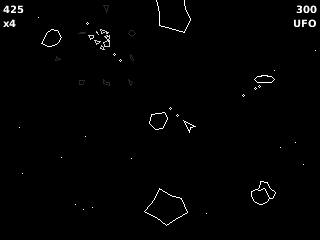
\includegraphics[width=50mm]{images/asteroids.png}}
\end{wrapfigure}

Let me elaborate. There is a similar duality in physics, which either
points at some deep underlying principle, or tells us something about
how our minds work. Richard Feynman mentions this duality as an
inspiration in his own work on quantum electrodynamics.

There are two forms of expressing most laws of physics. One uses local,
or infinitesimal, considerations. We look at the state of a system
around a small neighborhood, and predict how it will evolve within the
next instant of time. This is usually expressed using differential
equations that have to be integrated, or summed up, over a period of
time.

Notice how this approach resembles imperative thinking: we reach the
final solution by following a sequence of small steps, each depending on
the result of the previous one. In fact, computer simulations of
physical systems are routinely implemented by turning differential
equations into difference equations and iterating them. This is how
spaceships are animated in the asteroids game. At each time step, the
position of a spaceship is changed by adding a small increment, which is
calculated by multiplying its velocity by the time delta. The velocity,
in turn, is changed by a small increment proportional to acceleration,
which is given by force divided by mass.

These are the direct encodings of the differential equations
corresponding to Newton's laws of motion:
\begin{align*}
F = m \frac{dv}{dt} \\
v = \frac{dx}{dt}
\end{align*}
Similar methods may be applied to more complex problems, like the
propagation of electromagnetic fields using Maxwell's equations, or even
the behavior of quarks and gluons inside a proton using lattice \acronym{QCD}
(quantum chromodynamics).

This local thinking combined with discretization of space and time that
is encouraged by the use of digital computers found its extreme
expression in the heroic attempt by Stephen Wolfram to reduce the
complexity of the whole universe to a system of cellular automata.

The other approach is global. We look at the initial and the final state
of the system, and calculate a trajectory that connects them by
minimizing a certain functional. The simplest example is the Fermat's
principle of least time. It states that light rays propagate along paths
that minimize their flight time. In particular, in the absence of
reflecting or refracting objects, a light ray from point $A$ to point $B$
will take the shortest path, which is a straight line. But light
propagates slower in dense (transparent) materials, like water or glass.
So if you pick the starting point in the air, and the ending point under
water, it's more advantageous for light to travel longer in the air and
then take a shortcut through water. The path of minimum time makes the
ray refract at the boundary of air and water, resulting in Snell's law
of refraction:
\begin{equation*}
\frac{sin(\theta_1)}{sin(\theta_2)} = \frac{v_1}{v_2}
\end{equation*}
where $v_1$ is the speed of light in the air and $v_2$ is
the speed of light in the water.

\begin{figure}[H]
\centering
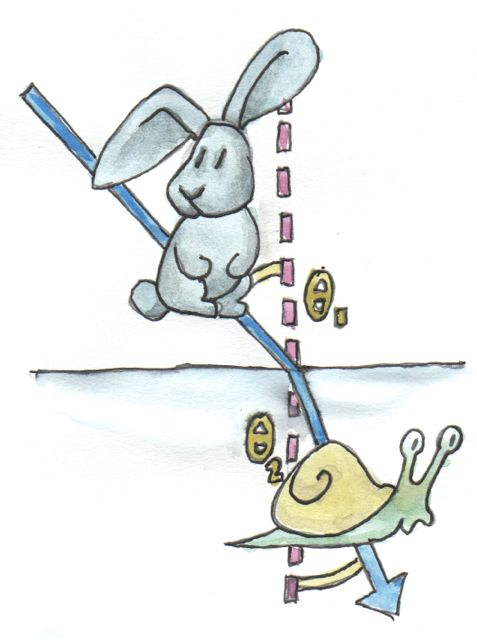
\includegraphics[width=1.56250in]{images/snell.jpg}
\end{figure}

All of classical mechanics can be derived from the principle of least
action. The action can be calculated for any trajectory by integrating
the Lagrangian, which is the difference between kinetic and potential
energy (notice: it's the difference, not the sum --- the sum would be
the total energy). When you fire a mortar to hit a given target, the
projectile will first go up, where the potential energy due to gravity
is higher, and spend some time there racking up negative contribution to
the action. It will also slow down at the top of the parabola, to
minimize kinetic energy. Then it will speed up to go quickly through the
area of low potential energy.

\begin{figure}[H]
\centering
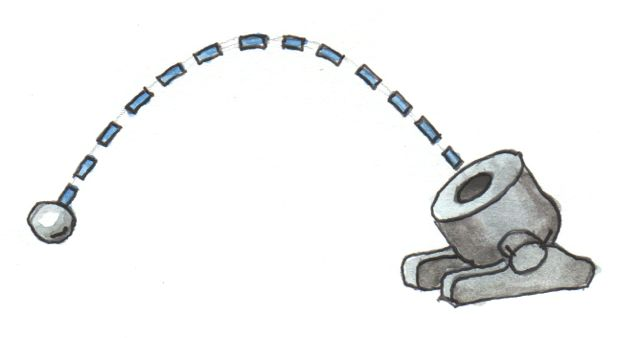
\includegraphics[width=1.56250in]{images/mortar.jpg}
\end{figure}

\noindent
Feynman's greatest contribution was to realize that the principle of
least action can be generalized to quantum mechanics. There, again, the
problem is formulated in terms of initial state and final state. The
Feynman path integral between those states is used to calculate the
probability of transition.

\begin{figure}[H]
\centering
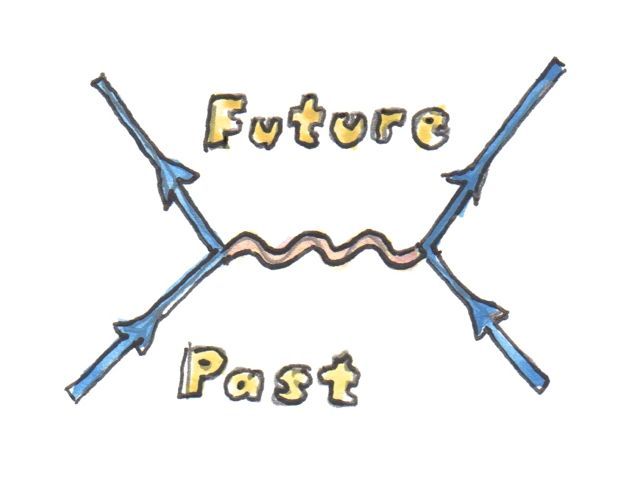
\includegraphics[width=1.56250in]{images/feynman.jpg}
\end{figure}

\noindent
The point is that there is a curious unexplained duality in the way we
can describe the laws of physics. We can use the local picture, in which
things happen sequentially and in small increments. Or we can use the
global picture, where we declare the initial and final conditions, and
everything in between just follows.

The global approach can be also used in programming, for instance when
implementing ray tracing. We declare the position of the eye and the
positions of light sources, and figure out the paths that the light rays
may take to connect them. We don't explicitly minimize the time of
flight for each ray, but we do use Snell's law and the geometry of
reflection to the same effect.

The biggest difference between the local and the global approach is in
their treatment of space and, more importantly, time. The local approach
embraces the immediate gratification of here and now, whereas the global
approach takes a long-term static view, as if the future had been
preordained, and we were only analyzing the properties of some eternal
universe.

Nowhere is it better illustrated than in the Functional Reactive
Programming (\acronym{FRP}) approach to user interaction. Instead of writing separate
handlers for every possible user action, all having access to some
shared mutable state, \acronym{FRP} treats external events as an infinite list,
and applies a series of transformations to it. Conceptually, the list of
all our future actions is there, available as the input data to our
program. From a program's perspective there's no difference between the
list of digits of $\pi$, a list of pseudo-random numbers, or a list of mouse
positions coming through computer hardware. In each case, if you want to
get the $n^\text{th}$ item, you have to first go through the first $n-1$ items. When
applied to temporal events, we call this property \emph{causality}.

So what does it have to do with category theory? I will argue that
category theory encourages a global approach and therefore supports
declarative programming. First of all, unlike calculus, it has no
built-in notion of distance, or neighborhood, or time. All we have is
abstract objects and abstract connections between them. If you can get
from $A$ to $B$ through a series of steps, you can also get there in one
leap. Moreover, the major tool of category theory is the universal
construction, which is the epitome of a global approach. We've seen it
in action, for instance, in the definition of the categorical product.
It was done by specifying its properties --- a very declarative
approach. It's an object equipped with two projections, and it's the
best such object --- it optimizes a certain property: the property of
factorizing the projections of other such objects.

\begin{figure}[H]
\centering
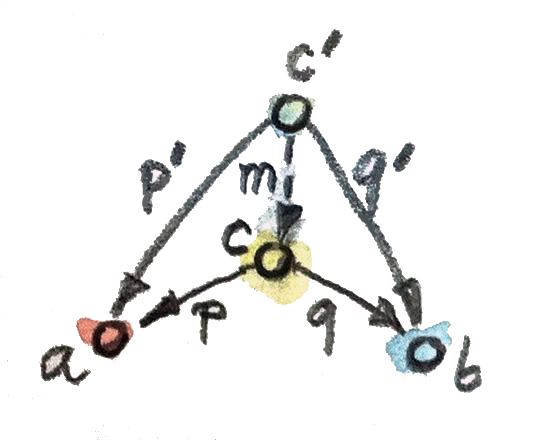
\includegraphics[width=1.56250in]{images/productranking.jpg}
\end{figure}

Compare this with Fermat's principle of minimum time, or the principle
of least action.

Conversely, contrast this with the traditional definition of a cartesian
product, which is much more imperative. You describe how to create an
element of the product by picking one element from one set and another
element from another set. It's a recipe for creating a pair. And there's
another for disassembling a pair.

In almost every programming language, including functional languages
like Haskell, product types, coproduct types, and function types are
built in, rather than being defined by universal constructions; although
there have been attempts at creating categorical programming languages
(see, e.g.,
\urlref{http://web.sfc.keio.ac.jp/~hagino/thesis.pdf}{Tatsuya
Hagino's thesis}).

Whether used directly or not, categorical definitions justify
pre-existing programming constructs, and give rise to new ones. Most
importantly, category theory provides a meta-language for reasoning
about computer programs at a declarative level. It also encourages
reasoning about problem specification before it is cast into code.